% State space diagram of the vector autoregressive model (vignette var).
\documentclass[tikz, border = 6pt]{standalone}
\usepackage{amsmath}
\usepackage{bm}
\usetikzlibrary{arrows.meta, positioning, calc}
\tikzset{
  lat/.style = {circle, draw, thick, minimum size = 13mm, inner sep = 0pt},
  obs/.style = {rectangle, draw, thick, minimum size = 11mm, inner sep = 1pt},
  noise/.style = {circle, draw, minimum size = 8mm, inner sep = 0pt},
  reg/.style = {-{Stealth[length = 2.5mm]}, thick},
  cov/.style = {{Stealth[length = 2mm]}-{Stealth[length = 2mm]}},
  var/.style = {cov, looseness = 5},
  lab/.style = {font = \footnotesize, fill = white, inner sep = 1pt},
  mat/.style = {font = \small, inner sep = 2pt, align = left},
  dots/.style = {font = \Large}
}
\begin{document}
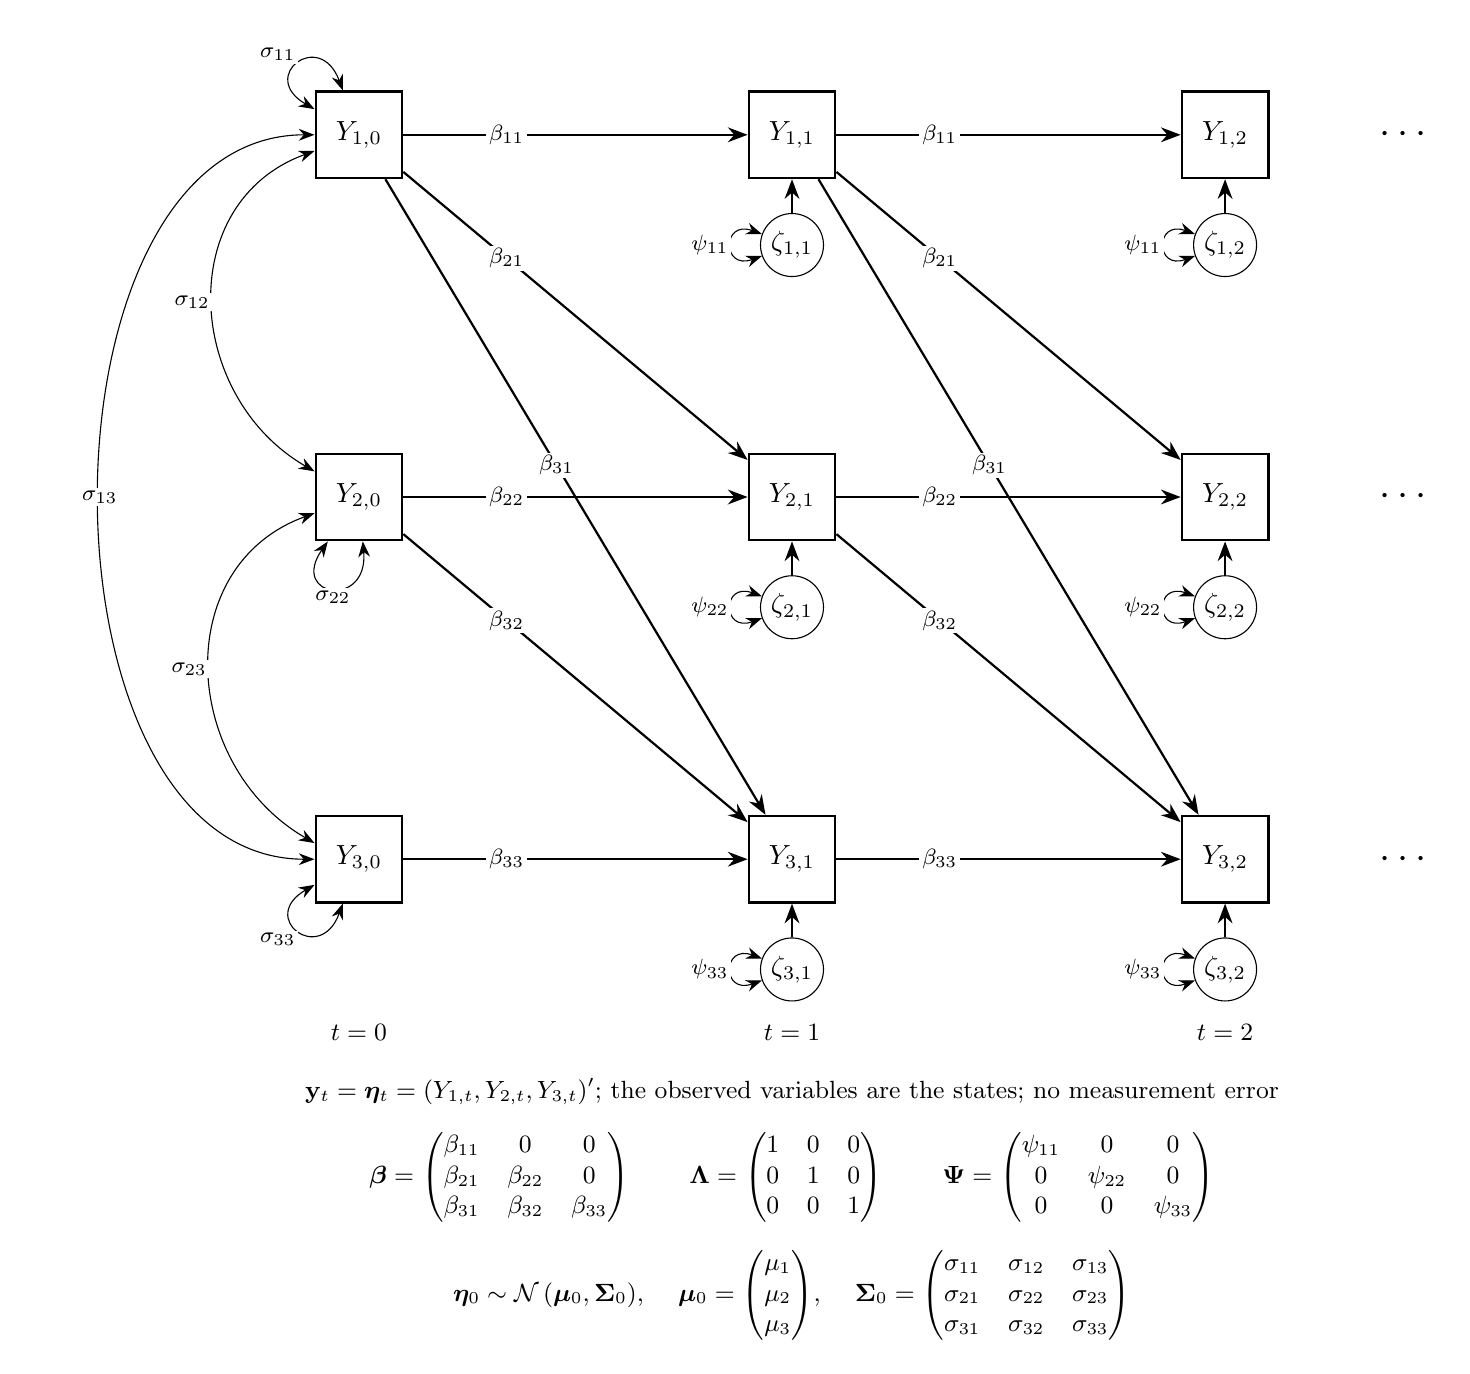
\begin{tikzpicture}
  % occasions: the observed variables are the states
  \foreach \t/\x in {0/0, 1/5.5, 2/11} {
    \foreach \j/\r in {1/0, 2/-4.6, 3/-9.2} {
      \node[obs] (e\j\t) at (\x, \r) {$Y_{\j, \t}$};
    }
    \node[font = \small] at (\x, -11.4) {$t = \t$};
  }
  % transitions
  \foreach \s/\t in {0/1, 1/2} {
    \foreach \j in {1, 2, 3} {
      \draw[reg] (e\j\s) -- node[lab, pos = 0.3] {$\beta_{\j\j}$} (e\j\t);
    }
    \draw[reg] (e1\s) -- node[lab, pos = 0.3] {$\beta_{21}$} (e2\t);
    \draw[reg] (e1\s) -- node[lab, pos = 0.45] {$\beta_{31}$} (e3\t);
    \draw[reg] (e2\s) -- node[lab, pos = 0.3] {$\beta_{32}$} (e3\t);
  }
  % process noise
  \foreach \t/\x in {1/5.5, 2/11} {
    \foreach \j/\r in {1/0, 2/-4.6, 3/-9.2} {
      \node[noise] (z\j\t) at (\x, \r - 1.4) {$\zeta_{\j, \t}$};
      \draw[reg] (z\j\t) -- (e\j\t);
      \draw[var] (z\j\t.160) to[out = 160, in = 200]
        node[lab, left] {$\psi_{\j\j}$} (z\j\t.200);
    }
  }
  \foreach \r in {0, -4.6, -9.2} {
    \node[dots] at (13.3, \r) {$\cdots$};
  }
  % initial condition
  \draw[var] (e10.110) to[out = 110, in = 150]
    node[lab, above left] {$\sigma_{11}$} (e10.150);
  \draw[var] (e20.235) to[out = 235, in = 275]
    node[lab, below] {$\sigma_{22}$} (e20.275);
  \draw[var] (e30.210) to[out = 210, in = 250]
    node[lab, below left] {$\sigma_{33}$} (e30.250);
  \draw[cov] (e10.200) to[out = 200, in = 150, looseness = 1.2]
    node[lab, left] {$\sigma_{12}$} (e20.150);
  \draw[cov] (e20.200) to[out = 200, in = 150, looseness = 1.2]
    node[lab, left] {$\sigma_{23}$} (e30.160);
  \draw[cov] (e10.west) .. controls (-4.2, 0) and (-4.2, -9.2) ..
    node[lab] {$\sigma_{13}$} (e30.west);
  % matrices
  \node[mat, align = center, below] at (5.5, -11.9) {%
    $\mathbf{y}_{t} = \bm{\eta}_{t} = \left( Y_{1, t}, Y_{2, t}, Y_{3, t}
      \right)^{\prime}$; the observed variables are the states;
    no measurement error \\[3mm]
    $\bm{\beta} = \begin{pmatrix}
      \beta_{11} & 0 & 0 \\
      \beta_{21} & \beta_{22} & 0 \\
      \beta_{31} & \beta_{32} & \beta_{33}
    \end{pmatrix}$
    \qquad $\bm{\Lambda} = \begin{pmatrix}
      1 & 0 & 0 \\ 0 & 1 & 0 \\ 0 & 0 & 1
    \end{pmatrix}$
    \qquad $\bm{\Psi} = \begin{pmatrix}
      \psi_{11} & 0 & 0 \\ 0 & \psi_{22} & 0 \\ 0 & 0 & \psi_{33}
    \end{pmatrix}$ \\[3mm]
    $\bm{\eta}_{0} \sim \mathcal{N} \left( \bm{\mu}_{0},
      \bm{\Sigma}_{0} \right)$, \quad
    $\bm{\mu}_{0} = \begin{pmatrix}
      \mu_{1} \\ \mu_{2} \\ \mu_{3}
    \end{pmatrix}$, \quad
    $\bm{\Sigma}_{0} = \begin{pmatrix}
      \sigma_{11} & \sigma_{12} & \sigma_{13} \\
      \sigma_{21} & \sigma_{22} & \sigma_{23} \\
      \sigma_{31} & \sigma_{32} & \sigma_{33}
    \end{pmatrix}$};
\end{tikzpicture}
\end{document}
